Uit de wandcontactdoos komt 230 Vac. Dat is de spanning\index{Spanning}, of het potentiaalverschil\index{Potentiaalverschil}. AA penlite batterijen hebben een spanning van 1,5 Vdc.

Als we de vergelijking maken met water, dan is de spanning vergelijkbaar met de druk. Als we een emmer met water op een trap zetten en in die emmer met water zit aan de onderkant een kraantje, dan staat er een bepaalde druk op de uitgang van de kraan. Als we de kraan dicht laten gebeurd er niets en toch is er die druk. Draaien we de kraan open dan stroomt er water. Zolang de emmer niet leeg is blijft er druk staan op het water. Zo werkt een batterij ook. Zolang als er spanning in de batterij zit kan er stroom lopen. Is de batterij leeg, dan is er geen spanning meer en ook geen stroom.

Het symbool voor de spanning is de U\index{U} en de eenheid is de V\index{V}, ofwel de Volt\index{Volt}. Voor de AA penlite batterij geldt dus: \[ U = 1,5 V \].

Achter de V kan een toevoeging komen, namelijk ac of dc. Deze termen zijn afkortingen en staan voor Alternating Current\index{Alternating Current}\index{AC} en Direct Current\index{Direct Current}\index{DC}. Of wel wissel stroom en gelijk stroom. AC en DC zijn Engelse termen. In het Nederlands spreken we wisselspanning of gelijkspanning terwijl we wel de afkortingen ac en dc gebruiken.

Bij een gelijkspanning\index{Gelijkspanning} blijft de 'druk' constant. Een batterij heeft een gelijkspanning. De batterij zal, als hij niet leeg is, continue een spanning hebben van 1,5 Volt.

Een wisselspanning\index{Wisselspanning} heeft, zoals de naam al aangeeft, een wisselende spanning. De spanning beweegt van het maximum, via de 0 naar een minimum en weer terug via een sinus-vorm, zie \ref{fig:sinus}.

\begin{figure}[h]
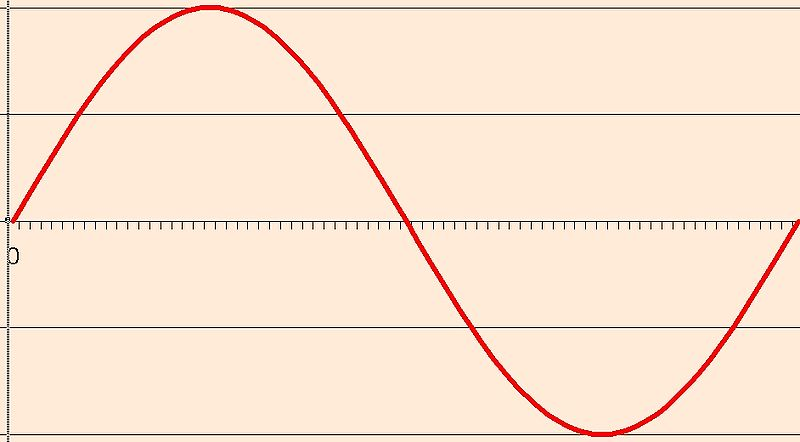
\includegraphics[width=5cm]{800px-Sinus}
\centering
\caption{Tekening door Philip Bosma (\url{https://commons.wikimedia.org/wiki/File:Sinus.jpg})}
\label{fig:sinus}
\end{figure}

De spanning uit het stopcontact maakt deze beweging 50 keer per seconde en heeft dus een frequentie van 50 Hz.

